Now that your can import your modelled concentration into ArcGIS, you
have access to all the available toolboxes.  In this section, we are
going to briefly show an example of how one might evaluate their
modelled concentration to observations.

\section{Generating Fake Observations}

If you have observations to evaluate your model outputs, great!
Otherwise, for the sake of this learning module we are going to
generate fake observations.  Because this section is outside the scope
of this learning module, it will be briefer than other sections.  If
you wish, there is a random points shape file in the included
material.

First, lets create a random point shape file.  To do this, open the
\textbf{Data Management Tools} $\rightarrow$ \textbf{Feature Class}
$\rightarrow$ \textbf{Create Random Points} tool.  Leave the optional
\emph{Constraining Feature Class (optional)} input empty, and instead
select your \emph{cmaq\_36} grid for the \emph{Constraining Extent
(optional)}.  Fill the remaining settings out as you see fit.

\subsection{Faking Realistic Data}
\label{faking_data}

This will provide you with a feature of points at random locations
within your area of interest.  These points however have no
data associated with them.  For realistic data, we will extract
concentration information from the raster layer at these points.
Once extracted, will will use the field calculator to add a random
signal to the concentrations thereby generating ``realistic looking''
data.

Open the \textbf{Spatial Analyst Tools} $\rightarrow$
\textbf{Extraction} $\rightarrow$ \textbf{Extract Values to Points}
tool.  Select your random points shape file as the \emph{Input point
features}, your raster file as the \emph{Input Raster} and choose a
place to output the shapefile.

In this new shapefile, open the \emph{Attribute Table}, add a new
field named \emph{O3\_obs} with a precision of 10 and scale of 8.
First, lets set the \emph{ID} to something usable (perhaps for future
joining). Open the field calculator on the \emph{ID} column and enter
the following formula,

\singlespace
\begin{minted}{python}
!FID!
\end{minted}
\doublespace

Now, open the field calculator on the new \emph{O3\_obs} column, in
the \emph{Pre-Logic Script Code} enter:
\singlespace
\begin{minted}{python}
import random
def addnoise(val):
   val = val * (1 + random.randint(-10,10)/10)
   return val
\end{minted}
\doublespace
\noindent Then in the \emph{O3\_obs = } text area, enter:
\singlespace
\begin{minted}{python}
addnoise( !RASTERVALU! )
\end{minted}
\doublespace

Delete the columns you do not need (\emph{RASTERVALUE}, etc).  And
\emph{voila}, you have realistic looking observations for all your
points.

\section{Evaluating Your Data}

There are many tools available in ArcGIS to compare your modelled data
to observation.  These tools can be as simple as point by point
comparison, or as complex as reading information from several sources
at once (say population, and land type, and \ldots)  In this section,
we will generate a scatter plot to compare the performance of our
modelled ozone concentration to observed concentration.  Note, in this
section we are assuming that time is not a factor, \ie~that the
modelled concentration displaying and the observational data we have
happen to be for the same time.

Add your observations to the data frame.  Your frame should appear
similar to figure \ref{observations}.

\begin{figure}
	\centering
	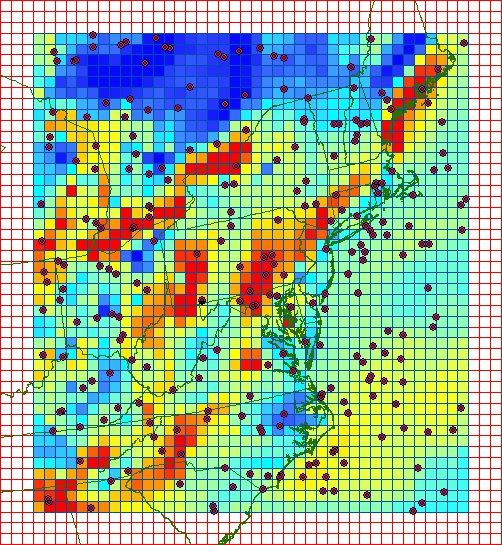
\includegraphics[width=0.6\textwidth]{observations.jpg}
	\caption{Example of observation site}
	\label{observations}
\end{figure}

The first step is to extract your data from the raster file
corresponding to your observation sites.  We are going to repeat the
procedure that was given in section \ref{faking_data}.

Open the \textbf{Spatial Analyst Tools} $\rightarrow$
\textbf{Extraction} $\rightarrow$ \textbf{Extract Values to Points}
tool.  Select your observations point feature as the \emph{Input point
features}, your raster file as the \emph{Input Raster} and choose a
place to output the shapefile.

Open the attribute table for this tool, you will notice that it has
copied the columns off your observation data.  This feature saves us
the effort of joining the tables.

On the \emph{Table Options} button, select \emph{Create Graph\ldots}.
From here, you can create a myriad of different graph styles.  Figure
\ref{scatter} shows an example of a scatter plot of the observations
versus the modelled data.  If one were to interpret the data, they
would see that there is little correlation (if any), but considering
that this is faked data it really has no barring on the quality of our
model.

\begin{figure}
	\centering
	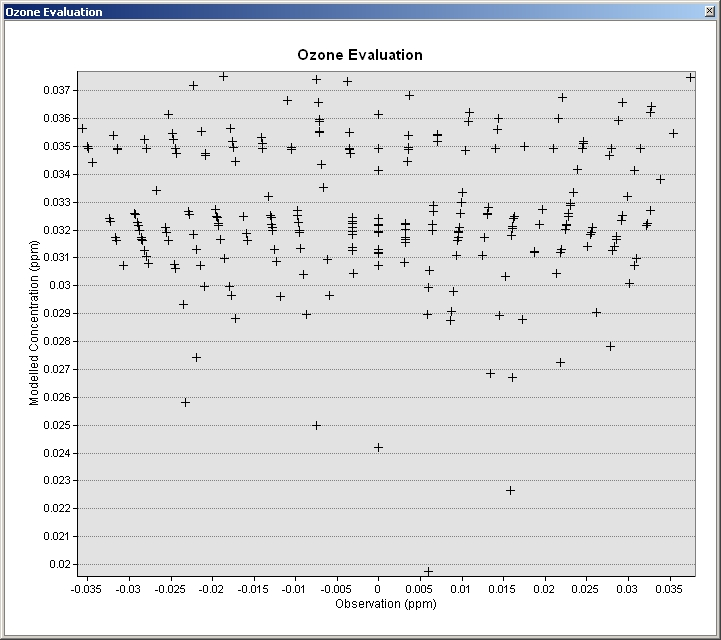
\includegraphics[width=0.6\textwidth]{eval_scatter_plot.jpg}
	\caption{Example of a scatter plot comparing observed ozone to
modelled ozone.}
	\label{scatter}
\end{figure}

To summarize, with the \textbf{Make IOAPI Raster File} tool, one can
now import \ioapi~output files from \ac{cmaq} and other \acp{aqm} into
ArcGIS where they have a full and matured set of analysis tools.
